\documentclass[12pt]{article}
\usepackage[english]{babel}
\usepackage{a4wide}             % Voor wat beter gevulde A4-tjes
\usepackage[utf8]{inputenc}     
\usepackage{graphicx}           % To add pictures
\usepackage{wrapfig}
\usepackage[hmargin=3cm,vmargin=3.5cm]{geometry}
\usepackage{caption}            % For better captions
\usepackage{pdfpages}           % To add PDF pages
\usepackage{color}              % For colored text
\usepackage{subcaption}         % For subcaptions
\usepackage{amssymb}  
\usepackage{fancyhdr}
\usepackage{amsmath}
\usepackage[export]{adjustbox}
\usepackage{titling}
\usepackage{eurosym}
\usepackage{times}
\usepackage{textcomp}
\usepackage{colortbl}
\usepackage{eurosym}
\usepackage{hyperref}
\usepackage{lastpage}
\usepackage{fancyhdr}
\usepackage[modulo]{lineno}
\usepackage[ampersand]{easylist}
\usepackage{soul}
\usepackage{marginnote}
\usepackage[normalem]{ulem}
\usepackage{multicol} 
\usepackage{float}

% Use XeLaTeX Compliler!!
\usepackage{fontspec}
\setmainfont{Arial}

\pagestyle{fancy} 

\fancypagestyle{importedpages}{%
  \fancyhf{}% Clear header/footer
  \renewcommand{\headrulewidth}{0pt}% Remove header rule
  \renewcommand{\footrulewidth}{0pt}% Remove footer rule (default)
  \fancyfoot[C]{\raisebox{-3\baselineskip}[0pt][0pt]{\thepage}}% Lower page number into position
}

\hypersetup{colorlinks,%
	citecolor=black,%
	filecolor=red,%
	linkcolor=black,%
	urlcolor=black}

%Header 
\setlength{\voffset}{-0.5in}% Afstand van de top tot de header (+1 inch)
\setlength{\headheight}{110pt}% Hoogte van de header
\setlength{\headsep}{10pt}% Afstand tussen header en document


\fancyhead{}
\fancyfoot{}
\fancyhead[RO,R]{
\includegraphics[width=250pt]{ETVLogoRCMYK.pdf}}
\fancyfoot[CO,C]{page \thepage~of \pageref{LastPage}}
\renewcommand{\headrulewidth}{0pt}
\renewcommand{\footrulewidth}{0.4pt}


\begin{document}
\raggedright
\reversemarginpar

\begin{figure}[H]
	\centering
	
\includegraphics[width=0.7\textwidth]{../images/klushok-logo.pdf} % comment when printing in black and white
\end{figure}

\begin{center}
	\LARGE{PCB workshop}\\
	\large{\today}\\
	\normalsize{Bram den Ouden}\\
	% ~\\
	% \large{\emph{Klushok - Electrotechnische Vereeniging}}\\
\end{center}




\section{Introduction}

Hey there and welcome to the klushok workshop!
This workshop is intended for absolute beginners and will guide you through making your very first PCB.
The software we'll be using is:
\begin{itemize}
	\item Kicad v6: \url{https://www.kicad.org/}
	\item Inkscape: \url{https://inkscape.org/}
	\item falstad circuit simulator: \url{https://www.falstad.com/circuit/circuitjs.html}
\end{itemize}

\textbf{KiCad} is a free and open source PCB design tool with similar functions to paid competitors like eagle and altium. It is actively maintained and there is a large community which helps new users or issues. Since Kicad is open source its users will always be able to open/edit older projects.

\textbf{Inkscape} is another open source firmware. It is used to design vector graphics and can be compared to adobe illustrator.

\textbf{Falstad} is a javascript tool which can accurately and visually simulate the operation of basic circuits. \\
\vspace{2ex}
We highly suggest you download and install Kicad and Inkscape whilst reading through this manual.

\subsection{Design choices}
During the design process of a PCB countless large and small changes will have to be made, these are left to the participant of the workshop. Some of the choices you should keep in mind whilst reading through this manual are:

\begin{itemize}
	\item How many LEDs will you add to the design
	\item How will you controll these LEDs
	\item What is the power source and expected input voltage
	\item Will you use surface mount (SMD) or through hole (THT) components
	\item What is the maximum/minimum size of the PCBs
\end{itemize}

\subsection{Workflow}
% Stukje over hoe PCB design een iteratief proces is en je op geen enkel moment moet twijfelen om een stap terug te zetten als dat de volgende stap makkelijker kan maken
% stappen in deze handleiding zijn gebaseerd op snelheid: falstad is sneller dan schematics en door de simulatie vis je 'domme' fouten er snel uit, pcb routen is trager dan schematics en is dus de laatste stap

Designing a PCB is not a linear progression. Each next step might result in having to make small adjustments in earlier steps. In general a step which simplifies a task in the next step is worth the iteration since the steps are built to be progressive in time consumption:
A falstad simulation consumes time in the order of minutes to 1 hour due to simplifications like replacing all LEDs with a single current source or resistor. The next step would be creating the schematics which can take up to multiple hours depending on complexity of the circuit. The final step in the process is placing components and routing the traces. This step can take anywhere between hours and days depending on complexity and size of the PCB since each simplification made in earlier steps has to be routed manually whilst keeping all copper and components surrouding your module in mind.

The steps presented in this manual will follow a time increasing order:
\begin{enumerate}
	\item First you will simulate your circuit to filter out any small mistakes and obtain values for your components. Simulations can also help to find critical points in your circuit. An example: which component becomes critical with a change in supply voltage?
	\item A schematic must implement many components which could be left out in simulations. A certain load could be replaced with a resistor in simulations but will have to be replaces by those, for example, 20 leds in the schematics. There is still some simplification possible by using hierarchical sheets for repeated modules and copy-pasting components. This stage can often be sped up by using the recommended schematics provided by most datasheets.
	\item The last step is creating the actual PCB. This step requires the user to layout all copper wires according to the connections described by the schematics. This step leaves very little room for copy-paste or repeated modules and is thus often the most time demanding step.
\end{enumerate}





\section{Schematics}
\textbf{Schematics} are block diagrams of an electrical circuit. \textbf{Components} are represented by blocks with one or more \textbf{pins}. Each pin represents a metal legs of a component to which something can be soldered. The connection between multiple pins is called a \textbf{net}. Each pin connected to the same net is considered to be electrically connected.

\textbf{Net labels} can be used to connect two nets without actually drawing the wires. Using these in just the right amount is an art on itself but greatly improves readabillity of schematics.
Besides connecting pins, net labels can also be used to name a net. This can be usefull when defining the copper wires on the PCB.

Schematics also allow thicker wires called \textbf{busses} to be used. These contain many wires which don't have to be drawn individually and can be used to greatly improve readabillity.


\subsection{Circuit}
% https://www.electronics-tutorials.ws/waveforms/astable.html

The circuit we will design will blink leds at a configurable speed and duty cycle. The basis of this circuit is an astable multivibrator.
Astable indicates that the circuit does not have a stable position, multivibrator suggests it will oscillate multiple outputs.

These suggestions are exactly what the circuit does: It has no stable position and will therefore keep oscillating.
Figure \ref{fig:astablemultivibrator} shows a basic configuration of such a circuit. Output 1 and 2 contain a square wave which can be used to drive single LEDs or LED drivers. Details of how this circuit works can be found on \url{https://www.electronics-tutorials.ws/waveforms/astable.html} and you're strongly advised to read this before continuing.

\begin{figure}[H]
	\centering
	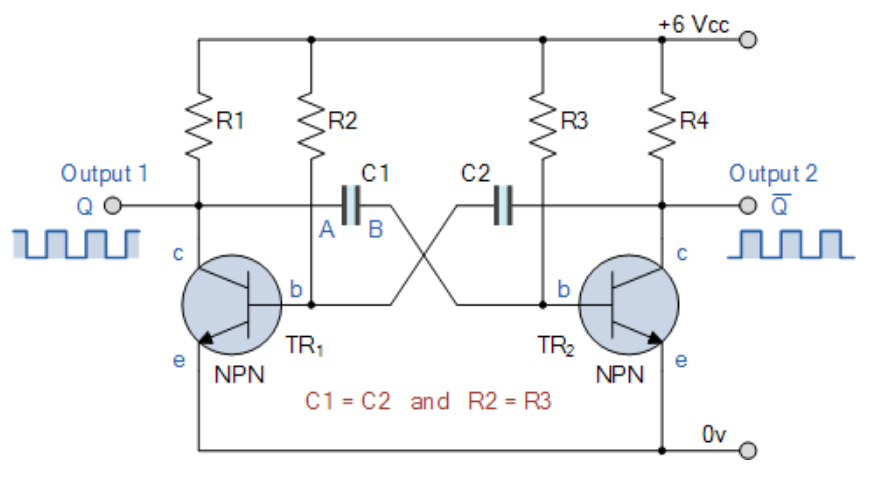
\includegraphics[width=0.7\textwidth]{../images/astablemultivibrator.png}
	\caption{Astable multivibrator. Source: \url{https://www.electronics-tutorials.ws/waveforms/astable.html}}
	\label{fig:astablemultivibrator}
\end{figure}

Besides the oscillator implemented by the astable multivibrator some LED drivers are required. These LED drivers are added to ensure that the behaviour of the LEDs does not influence the oscillator.
Depending on the outcome of the earlier mentioned design choices there are different ways to implement LED drivers: A higher input voltage may allow driving multiple LEDs in series whilst lower input voltages (like when using a coin cell battery) will require driving the LEDs in parallel with individual resistors.

When deciding on the configuration of the LEDs, the switching element itself must also be considered:
A BJT requires no extra components and since it operates on current, its behaviour is less dependent on supply voltage. A MOSfet can switch large currents but requires a gate-source voltage higher than its treshold value.

A quick way to validate your design is to use the Falstad Circuit Simulator mentioned earlier. It is highly advised to have all critical parts simulated in falstad before moving on to Kicad.

\subsection{Creating a Kicad project}
To create a new KiCad project first open KiCad 6. A screen similar to figure \ref{fig:kicad_main} will appear. Go to the main screen and click on 'file'->'New Project' to create a project. An explorer window pops up asking for a location and a name. Keep in mind that when making a project, KiCad will create a folder with the same name as a project directory. Click 'save' and you will now see a file tree appear with your project name, a kicad\_sch file and a kicad\_pcb file. The sch file will contain your schematics and the pcb file will contain the PCB. On the right side of the window there are many more options which are not needed for this very first PCB we will create. 

\begin{figure}[h]
	\centering
	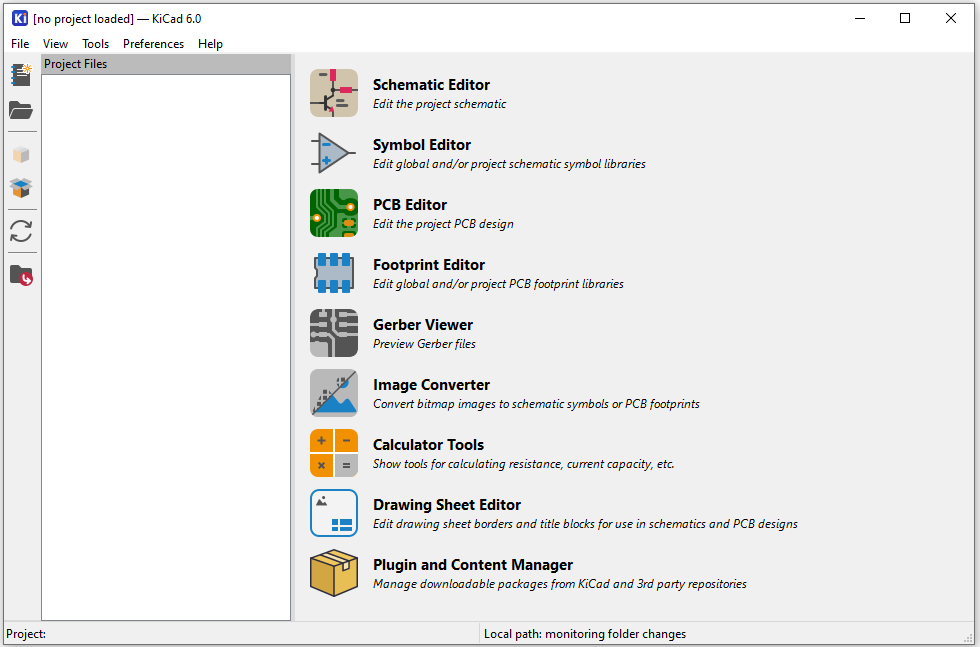
\includegraphics[width=.9\textwidth]{../images/kicad_main.png }
	\caption{}
	\label{fig:kicad_main}
\end{figure}



\subsection{Creating schematics}
Double click on the kicad\_sch file in the file tree to open the schematic editor. An empty layout will appear in addition to a side- and top bar as shown in figure \ref{fig:schematic_editor}. 

Click on the op-amp icon in the right side bar to add components (shortcut 'a'), the first time you click this it might take some time to open.\\
Search for 'R' to add a generic resistor, click once on a result to see the schematic or double click a result to place it. The resistor will be stuck to your cursor until you click, which will place it. 
Repeat this process until all required components are placed.\\\vspace{1ex}

\textbf{Note:} For the transistor you will need to select a specific model, check availabillity on \url{https://klushok.etv.tudelft.nl/inventory/components} or use the 2N3904 as a default NPN transistor.
\\\vspace{2ex}

\begin{figure}[H]
	\centering
	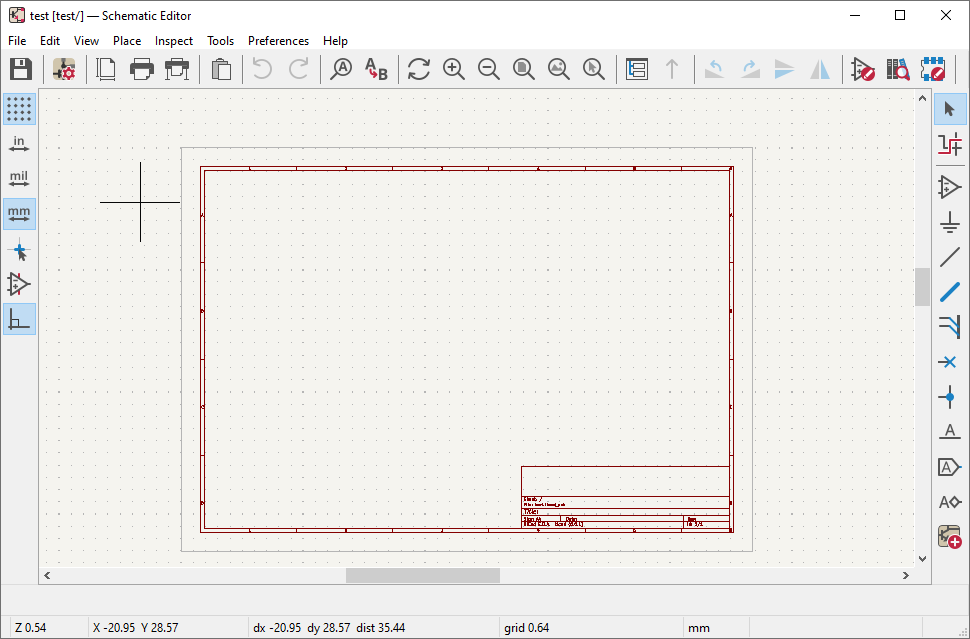
\includegraphics[width=0.9\textwidth]{../images/schematic_editor.png}
	\caption{KiCad schematic editor}
	\label{fig:schematic_editor}
\end{figure}



\subsubsection{Basic commands}
Left click a component to select it, click again to drag the component.
The value and identifier of a component can be moved by clicking the identifier or value and dragging them.
Right click and hold to move your view across the schematic. 
Scroll to zoom in or out and click left and hold to select multiple components.
By selecting a component and rightclicking them you can open an action menu. 
Go to properties in this action menu to adjust multiple parameters such as the associated footprint, value or datasheet link. All options have their keyboard shortcut listed next to them.\\
Adding wires can be done by clicking on the thin stripe in the sidebar of the schematic editor, pressing 'w' on the keyboard or by clicking the pins which have circle around them. Use these wires to connect all placed components. Take your time to make sure the components are positioned in a logical order, use net labels where needed.

\subsubsection{Validation}
Once you've made the schematic, verify that it matches the simulated circuit and carefully double check no incorrect connections were made by for example crossing wires. 
Ask a committee member to double check if you're in doubt.


\section{PCB}
% two approaches: first create outline and fill in components or first lay components in desired pattern and then make outline around them

% discuss outline considerations and limitations based on manufacturer
\subsection{Keyboard shortcuts}
list of shortcuts or link to where these are listed


\subsection{Footprints}
not all devices have default Footprints
ensure the footprint matches the version of your symbol (2n3904 THT has a different pinout from the smd version for example).

select component, press e to open properties, click book icon in the footprint field to open footprint editor, select correct footprint. Do this for 1 of each type to make the next step easier.

now click the 'run footprint assignment tool' button in the top bar of the schematic editor. If you have not already done so, a popup will ask you to annotate the schematics. Annotation means replacing the questionmarks in the device identifiers by numbers.

\begin{figure}[h]
	\centering
	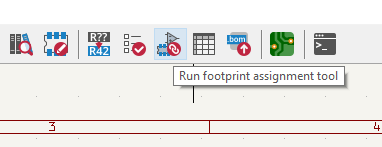
\includegraphics[width=0.5\textwidth]{../images/run_footprint_assignment_tool.png}
	\caption{}
	\label{fig:run_footprint_assignment_tool}
\end{figure}


% battery footprint https://nl.farnell.com/multicomp-pro/mp000357/battery-holder-2032-smd/dp/3126595?st=cr2032%20holder



\subsection{PCB edge}
% wat is de edge, waarom is die belangrijk, wat zijn dingen om rekening mee te houden
% info stukje over handmatig een outline tekenen vs importeren (voordelen van aanpassen van maten en eventueel CAD programmas vermelden)
% introductie inkscape
Outline from svg:
\begin{enumerate}
	\item Open PCB editor
	\item File->import->graphics
	\item Select 'Edge.cuts' for option 'graphic layer' as shown in figure \ref{fig:outline_import}
	      \begin{figure}[H]
		      \centering
		      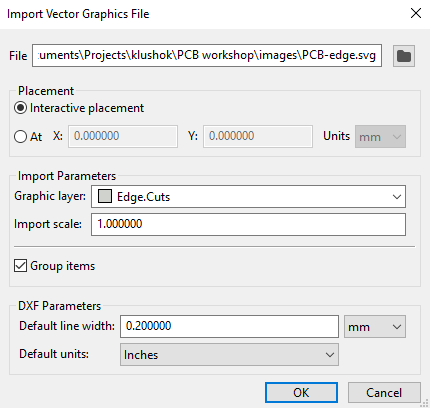
\includegraphics[width=0.7\textwidth]{../images/graphic_outline_import.png}
		      \caption{}
		      \label{fig:outline_import}
	      \end{figure}
	\item Select the vector file containing the desired outline
	\item Drag the outline to the desired location and click to place
	\item Open the 3D viewer (alt + 3) to verify that the outline has been placed correctly
\end{enumerate}

\subsection{Placing components}
Import the design made in the schematic editor by clicking the "update pcb" button shown in figure \ref{fig:update_pcb}. This will import all components with their assigned footprints to the PCB editor. Place them somewhere next to your previously defined board edge. The components are connected using thin wires which are called the ratsnest. These lines indicate the shortest path between two pins of a single node and must eventually be replaced by copper traces.

\begin{figure}[h]
	\centering
	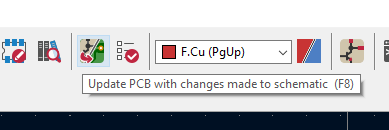
\includegraphics[width=0.5\textwidth]{../images/update_PCB.png}
	\caption{}
	\label{fig:update_pcb}
\end{figure}

Drag individual components to the location you'd like on the PCB. Start with large or very important components, end with smaller stuff like resistors. Through hole components have a copper pad on both sides of the PCB which is something you should keep in mind when placing them next to surface mount components.
Although components can be placed on both sides of the PCB, soldering becomes a lot easier if you keep them to a single side.

Once the components are generally in the location you'd like, check if the ratsnest shows feasible routes, try to rotate components to have a minimally tangled ratsnest.




\section{Conclusion}
This workshop has tought you how to create a PCB but the most important part of making the actual PCB is experience. Each step can take anywhere from minutes to hours depending on de complexity of the circuit and how well the designer can separate the complete design in smaller blocks with nicely placed ports.

We hope you had a great first experience with designing PCBs and many more will follow. Feel free to ask members of the klushok committee for advise at any time, we all like to help!

Thank you for participating and we hope to see you on future workshops!\\
\vspace{3ex}
\textit{The Klushok committee}

\end{document}


